\subsection{Tìm kiếm các bài đăng tải nhà thuê}
\subsubsection{Sơ đồ use-case}
\begin{figure}[H]
    \centering
    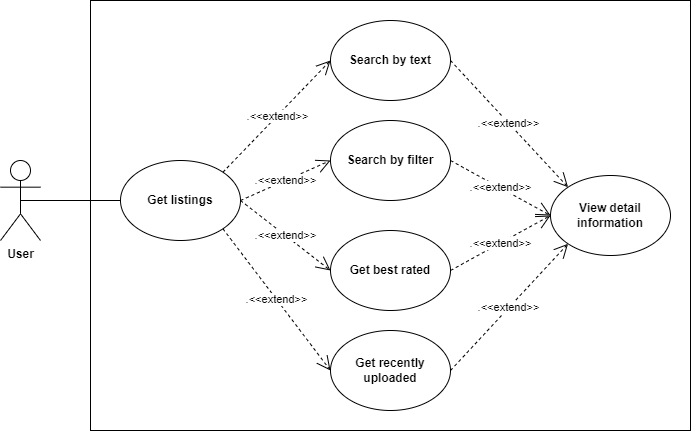
\includegraphics[width=1\textwidth]{Images/UseCase/GetListing.png}
    \caption{Sơ đồ use-case cho các chức năng liên quan đến tìm kiếm các bài đăng tải nhà thuê}
\end{figure}
\subsubsection{Đặc tả use-case cho chức năng tìm kiếm bài đăng nhà thuê bằng văn bản}
\begin{center}
    \arrayrulecolor{cyan!75!black}
    \arrayrulewidth=2pt
    \begin{longtable}{
        |>{\raggedright\arraybackslash}p{3cm}
        |>{\raggedright\arraybackslash}p{13cm}
        |}
        \hline
        \rowcolor{cyan!75!black} \textcolor{white}{\textbf{Use-case name}} & \textcolor{white}{\textbf{TÌM KIẾM NHÀ THUÊ BẰNG VĂN BẢN}}
        \\\hline
        \rowcolor{cyan!10!white} \textit{Actor} & Người dùng
        \\\hdashline
        \rowcolor{cyan!10!white} \textit{Description} & Tính năng cho phép người dùng tìm kiếm danh sách các bài đăng nhà thuê dựa theo các mong muốn của người dùng bằng văn bản.
        \\\hdashline
        \rowcolor{cyan!10!white} \textit{Preconditions} & Không có
        \\\hdashline
        \rowcolor{cyan!10!white} \textit{Postconditions} & Kết quả tìm kiếm được trả về thành công dưới dạng danh sách các bài đăng nhà thuê.
        \\\hdashline
        \rowcolor{cyan!10!white} \textit{Trigger} & Người dùng chọn vào thanh tìm kiếm ở trên giao diện của ứng dụng.
        \\\hdashline
        \rowcolor{cyan!10!white} \textit{Main flow} &
        1. Người dùng gõ văn bản tìm kiếm và nhấn vào biểu tượng tìm kiếm. \newline
        2. Ứng dụng xử lý văn bản tìm kiếm và thực hiện truy vấn kết quả tìm kiếm. \newline
        3. Kết quả tìm kiếm được hiển thị trên giao diện.
        \\\hdashline
        \rowcolor{cyan!10!white} \textit{Alternative flow} & 
         \textbf{Nếu người dùng thoát khỏi chức năng tìm kiếm bằng văn bản, ứng dụng sẽ quay về màn hình chính} 
        1a.1. Người dùng hủy khi đang gõ văn bản tìm kiếm danh sách bài đăng nhà thuê. \newline
        1a.2. Ứng dụng quay trở về màn hình chính.
        \\\hdashline
        \rowcolor{cyan!10!white} \textit{Exception flow} &
        \textbf{Nếu ứng dụng gặp lỗi khi tìm kiếm bài đăng nhà thuê, ứng dụng thông báo lỗi và yêu cầu người dùng thử lại sau} \newline
        1a.1. Ứng dụng hiện lỗi khi thực hiện tìm kiếm bài đăng nhà thuê. \newline
        1a.2. Ứng dụng thông báo yêu cầu người dùng thử lại sau.
        \\\hline
        \caption{Đặc tả use-case cho chức năng tìm kiếm bài đăng nhà thuê bằng văn bản}
    \end{longtable}
\end{center}
\subsubsection{Đặc tả use-case cho chức năng tìm kiếm bài đăng nhà thuê bằng bộ lọc}
\begin{center}
    \arrayrulecolor{cyan!75!black}
    \arrayrulewidth=2pt
    \begin{longtable}{
        |>{\raggedright\arraybackslash}p{3cm}
        |>{\raggedright\arraybackslash}p{13cm}
        |}
        \hline
        \rowcolor{cyan!75!black} \textcolor{white}{\textbf{Use-case name}} & \textcolor{white}{\textbf{TÌM KIẾM NHÀ THUÊ BẰNG BỘ LỌC}}
        \\\hline
        \rowcolor{cyan!10!white} \textit{Actor} & Người dùng
        \\\hdashline
        \rowcolor{cyan!10!white} \textit{Description} & Tính năng cho phép người dùng tìm kiếm danh sách các bài đăng nhà thuê dựa theo các tiêu chí mong muốn của người dùng bằng bộ lọc.
        \\\hdashline
        \rowcolor{cyan!10!white} \textit{Preconditions} & Không có
        \\\hdashline
        \rowcolor{cyan!10!white} \textit{Postconditions} & Kết quả tìm kiếm được trả về thành công dưới dạng danh sách các bài đăng nhà thuê.
        \\\hdashline
        \rowcolor{cyan!10!white} \textit{Trigger} & Người dùng chọn vào bộ lọc tìm kiếm ở trên giao diện của ứng dụng.
        \\\hdashline
        \rowcolor{cyan!10!white} \textit{Main flow} &
        1. Người dùng lọc các tiêu chí tìm kiếm trên màn hình bộ lọc và nhấn vào biểu tượng tìm kiếm. \newline
        2. Ứng dụng thực hiện truy vấn kết quả tìm kiếm. \newline
        3. Kết quả tìm kiếm được hiển thị trên giao diện.
        \\\hdashline
        \rowcolor{cyan!10!white} \textit{Alternative flow} & 
         \textbf{Nếu người dùng thoát khỏi chức năng tìm kiếm bằng bộ lọc, ứng dụng sẽ quay về màn hình chính} 
        1a.1. Người dùng hủy khi đang sử dụng bộ lọc tìm kiếm danh sách bài đăng nhà thuê. \newline
        1a.2. Ứng dụng quay trở về màn hình chính.
        \\\hdashline
        \rowcolor{cyan!10!white} \textit{Exception flow} &
        \textbf{Nếu ứng dụng gặp lỗi khi tìm kiếm bài đăng nhà thuê, ứng dụng thông báo lỗi và yêu cầu người dùng thử lại sau} \newline
        1a.1. Ứng dụng hiện lỗi khi thực hiện tìm kiếm bài đăng nhà thuê. \newline
        1a.2. Ứng dụng thông báo yêu cầu người dùng thử lại sau.
        \\\hline
        \caption{Đặc tả use-case cho chức năng tìm kiếm bài đăng nhà thuê bằng bộ lọc}
    \end{longtable}
\end{center}
\subsubsection{Đặc tả use-case cho chức năng lấy danh sách nhà thuê được đánh giá tốt nhất hoặc đăng tải gần đây nhất}
\begin{center}
    \arrayrulecolor{cyan!75!black}
    \arrayrulewidth=2pt
    \begin{longtable}{
        |>{\raggedright\arraybackslash}p{3cm}
        |>{\raggedright\arraybackslash}p{13cm}
        |}
        \hline
        \rowcolor{cyan!75!black} \textcolor{white}{\textbf{Use-case name}} & \textcolor{white}{\textbf{LẤY DANH SÁCH NHÀ THUÊ ĐƯỢC ĐÁNH GIÁ TỐT NHẤT HOẶC ĐĂNG TẢI GẦN ĐÂY NHẤT}}
        \\\hline
        \rowcolor{cyan!10!white} \textit{Actor} & Người dùng
        \\\hdashline
        \rowcolor{cyan!10!white} \textit{Description} & Tính năng cho phép người dùng lấy ra được danh sách các bài đăng tải nhà cho thuê được đánh giá tốt nhất hoặc được đăng tải gần đây nhất.
        \\\hdashline
        \rowcolor{cyan!10!white} \textit{Preconditions} & Không có
        \\\hdashline
        \rowcolor{cyan!10!white} \textit{Postconditions} & Kết quả được trả về thành công dưới dạng danh sách các bài đăng nhà thuê.
        \\\hdashline
        \rowcolor{cyan!10!white} \textit{Trigger} & Người dùng đang ở giao diện màn hình chính của ứng dụng.
        \\\hdashline
        \rowcolor{cyan!10!white} \textit{Main flow} &
        1. Ứng dụng đang hiển thị giao diện màn hình chính. \newline
        3. Kết quả danh sách các bài đăng tải nhà thuê được đánh giá tốt nhất hoặc đăng tải gần đây nhất được hiển thị thành công trên giao diện.
        \\\hdashline
        \rowcolor{cyan!10!white} \textit{Alternative flow} & Không có
        \\\hdashline
        \rowcolor{cyan!10!white} \textit{Exception flow} &
        \textbf{Nếu ứng dụng gặp lỗi khi thực hiện lấy ra danh sách bài đăng tải nhà thuê, ứng dụng thông báo lỗi và yêu cầu người dùng thử lại sau} \newline
        1a.1. Ứng dụng hiện lỗi khi thực hiện lấy ra danh sách bài đăng tải nhà thuê. \newline
        1a.2. Ứng dụng thông báo yêu cầu người dùng thử lại sau.
        \\\hline
        \caption{Đặc tả use-case cho chức năng lấy danh sách nhà thuê được đánh giá tốt nhất hoặc đăng tải gần đây nhất}
    \end{longtable}
\end{center}
\subsubsection{Đặc tả use-case cho chức năng xem thông tin chi tiết về bài đăng tải nhà thuê}
\begin{center}
    \arrayrulecolor{cyan!75!black}
    \arrayrulewidth=2pt
    \begin{longtable}{
        |>{\raggedright\arraybackslash}p{3cm}
        |>{\raggedright\arraybackslash}p{13cm}
        |}
        \hline
        \rowcolor{cyan!75!black} \textcolor{white}{\textbf{Use-case name}} & \textcolor{white}{\textbf{XEM THÔNG TIN CHI TIẾT VỀ BÀI ĐĂNG NHÀ THUÊ}}
        \\\hline
        \rowcolor{cyan!10!white} \textit{Actor} & Người dùng
        \\\hdashline
        \rowcolor{cyan!10!white} \textit{Description} & Tính năng cho phép người dùng xem thông tin chi tiết về bài đăng tải nhà thuê.
        \\\hdashline
        \rowcolor{cyan!10!white} \textit{Preconditions} & Ứng dụng đang hiển thị theo dạng danh sách các bài đăng tải nhà thuê
        \\\hdashline
        \rowcolor{cyan!10!white} \textit{Postconditions} & Thông tin chi tiết về một bài đăng tải nhà thuê được hiển thị thành công trên ứng dụng.
        \\\hdashline
        \rowcolor{cyan!10!white} \textit{Trigger} & Người dùng chọn vào một bài đăng tải nhà thuê đang được hiển thị trên danh sách các bài đăng tải.
        \\\hdashline
        \rowcolor{cyan!10!white} \textit{Main flow} &
        1. Ứng dụng lấy ra các thông tin liên quan đến bài đăng tải nhà thuê. \newline
        2. Ứng dụng hiển thị thông tin chi tiết về bài đăng tải nhà thuê.
        \\\hdashline
        \rowcolor{cyan!10!white} \textit{Alternative flow} & Không có
        \\\hdashline
        \rowcolor{cyan!10!white} \textit{Exception flow} &
        \textbf{Nếu ứng dụng gặp lỗi khi hiển thị thông tin chi tiết của bài đăng tải nhà thuê, ứng dụng thông báo lỗi và yêu cầu người dùng thử lại sau} \newline
        1a.1. Ứng dụng hiện lỗi khi hiển thị lấy ra danh sách bài đăng tải nhà thuê. \newline
        1a.2. Ứng dụng thông báo yêu cầu người dùng thử lại sau.
        \\\hline
        \caption{Đặc tả use-case cho chức năng xem thông tin chi tiết về bài đăng tải nhà thuê}
    \end{longtable}
\end{center}